\begin{columns}[totalwidth=.85\linewidth]
	\column{\textwidth}

		\begin{itembox}[l]{せん断変形時の応答とヒステリシス}
			変形速度の異なるせん断変形($\dot{\gamma} = 1e^{-2} \sim 5^{e-5}$)時の SS カーブを、各種モデルの理論曲線と共に Fig. \ref{deform} に示した。
			変形速度の低減により、$\gamma<1$ 程度の小さなひずみでは PNM に漸近することが確認できた。

			PNM へと漸近する変形速度 ($\dot{\gamma} = 2e^{-4}$) で周期的な変形 ($\gamma = 1$) を付与した結果を示した (Fig. \ref{cyclic})。
			複数回の変形に対しても迅速な回復を伴った力学的ヒステリシス (Hysteresis loss $\simeq$ 0.34) を示すことが確認できた。
			\begin{columns}[totalwidth=\linewidth]
				\column{.5\textwidth}
				\begin{figure}[htb]
					\centering
						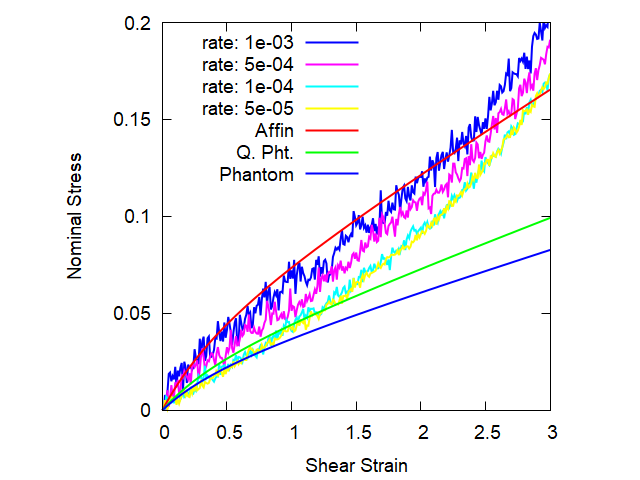
\includegraphics[width=.8\textwidth]{Shear_Random_4chain_N20.png}
						\caption{Strain Stress Curves for shear strain}
						\label{deform}
				\end{figure}
				\column{.5\textwidth}
				\begin{figure}[htb]
					\centering
						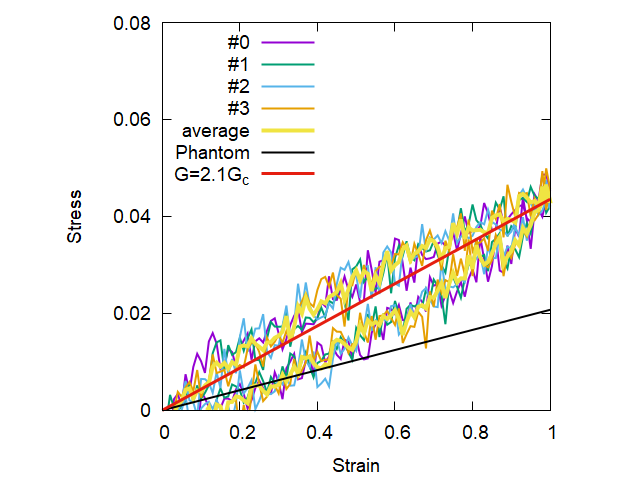
\includegraphics[width=.8\textwidth]{CyclicDeform_4chain_rate_2e-4.png}
						\caption{Hysteresis Response with Cyclic Deformations}
						\label{cyclic}
				\end{figure}
				\end{columns}
		\end{itembox}

		\begin{itembox}[l]{ヒステリシスロス}
			各種の変形条件での力学的ヒステリシスの振る舞いを、Fig. \ref{hystall}, \ref{hystallcomp} に示した。
			変形速度の低下に伴いヒステリシスロスは減少し、$\dot{\gamma} \sim 1e^{-5}$ 程度のオーダーの時間スケールで消失するようであった。
			\begin{columns}[totalwidth=\linewidth]
				\column{.5\textwidth}
					\begin{figure}[htb]
						\centering
							\includegraphics[width=\textwidth]{hyst_shear_all.png}
							\caption{Hysteresis losses for valid shear rate and maximum deformation}
							\label{hystall}
					\end{figure}
				\column{.5\textwidth}
				\begin{figure}[htb]
					\centering
						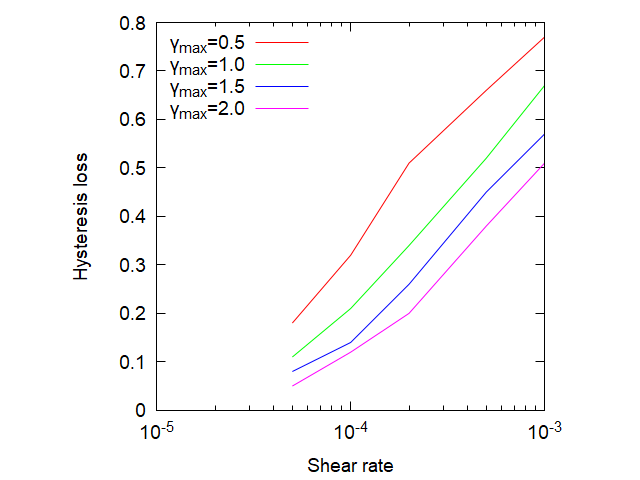
\includegraphics[width=.8\textwidth]{hyst_shear.png}
						\caption{Comparison of Hysteresis losses}
						\label{hystallcomp}
				\end{figure}
				\end{columns}
		\end{itembox}

		\begin{itembox}[l]{ヒステリシスロス}
			\begin{columns}[totalwidth=\linewidth]
				\column{.5\textwidth}
				ラウスモード(p=1)の自己相関関数 $C_p(t)$ から最長緩和時間 ($\tau$) を評価した (Fig. \ref{ac-xp}) 。
				\begin{align*}
					C_p(t) = \langle X_p(t)X_p(0) \rangle/\langle X_p^2 \rangle
				\end{align*}
				
				ネットワークのストランドは空間的に拘束されているためその相関は長時間極限で一定値に収束する。
				その値 $C_p(\infty)$ を差し引いて指数関数により緩和成分の評価を行い、$\tau \simeq 6.5e^{4}$ を得た。
				
				\column{.5\textwidth}
				\begin{figure}[htb]
					\centering
						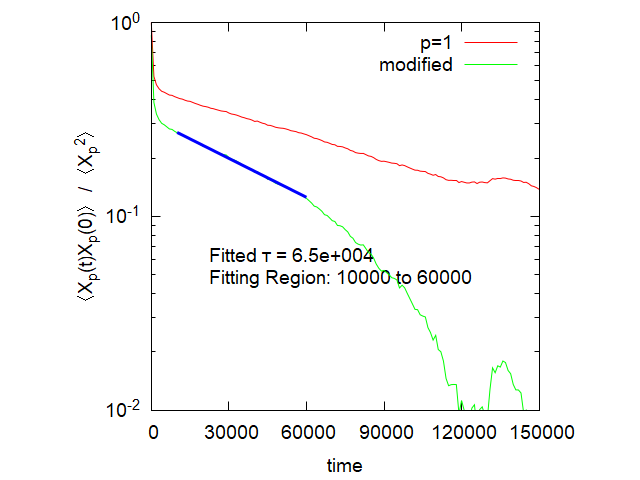
\includegraphics[width=.8\textwidth]{Xp_1_org.png}
						\caption{Auto Correlation of Rouse mode (p=1) for equilibrated structure}
						\label{ac-xp}
				\end{figure}
				\end{columns}
		\end{itembox}

\end{columns}